\chapter{Fundamentals}
\label{chap:nlp}

This chapter presents the fundamental knowledge necessary to understand the work and research done for this thesis.
Section \ref{sec:nlp} explains \ac{nlp} concepts like \acp{fnn}, training and optimization, tokenization, the transformer architecture and \ac{peft} techniques.
Section \ref{sec:metrics} presents various popular metrics used to evaluate code synthesis \acp{lm}.
Section \ref{sec:thestack} introduces the The Stack dataset, the basis for the TinyFuncData dataset created by this thesis.
Finally, section \ref{sec:basemodels} explores possible models that could serve as the base for TinyFuncCoder.

\section{Natural Language Processing}
\label{sec:nlp}
\Ac{nlp} is a field that has received much public attention since its inception.
From early chatbots like ELIZA \cite{Weizenbaum.1966} to Amazon's Alexa \cite{Kumar.2017}, Google Translate \cite{Wu.2016} or the recent breakthroughs in \acp{lm} like the ubiquitous transformer architecture \cite{Vaswani.2017} in 2017 and OpenAI's ChatGPT \cite{OpenAI.2022,AlecRadfordKarthikNarasimhanTimSalimansIlyaSutskever.2018,Brown.2020} in 2022.
\ac{nlp} has a vast amount of use cases, including content filters, text analysis, completion and prediction or translation.
Most relevant for this thesis is its use in code synthesis.
In essence, \ac{nlp} is a field of study in which computers learn to interact with natural language, as opposed to structured language like code.
It can be broadly split into \ac{nlu} and \ac{nlg}, the first of which processes natural language into an internal representation, and the second processes internal representations into natural language based on an input.

\subsection{History of NLP}
\label{sec:history}
The field of \ac{nlp} has existed since the 1950's, with three major epochs.
Symbolic \ac{nlp}, starting in the 50's \cite{Nadkarni.2011,Johri.2021}, working mostly with sets of hand-written rules and being rather limited in scope.
With Chomsky's introduction of syntactic structures \cite{Lees.1957}, computers could process simple phrases.
While many developments in the field had impressive capabilities for the time, it became apparent that natural language could not easily be captured in a structured language.
Natural language has a very large vocabulary and is ambiguous and reliant on context to process.

With ever-increasing computer processing power and the invention of \ac{ml}, \ac{nlp} adopted a statistical approach in the 90's \cite{Nadkarni.2011}.
It replaced the rigid rules of the symbolic method with statistical models that would predict the most likely word based on a previous series of words.
Models were trained on large bodies of annotated text \cite{Nadkarni.2011,Manning.1999}, utilizing the \ac{ml} practice of supervised learning.

This \ac{ml} approach was strengthened with the adoption of deep learning and neural networks.
In 2003, Bengio et al. introduced the foundation for most current \ac{nlp}, creating a neural model that handily outperformed the $n$-gram model, the best model at the time \cite{Bengio.2003}.
More recent advancements will be discussed in their own upcoming sections.

\subsection{Machine Learning Fundamentals}
\label{sec:ml}
This section will provide a brief overview of the underlying \ac{ml} concepts of current \ac{nlp} architecture, the \ac{fnn} and how optimizers are used in its training.

\subsubsection{Feedforward Neural Networks}
\label{sec:fnn}
A \ac{fnn}, broadly, is a collection of interconnected artificial neurons through which data flows and is processed.
An artificial neuron, inspired by a biological neuron, consists of a set of operations done on an input.
As shown in figure \ref{fig:neuron}, it consists of an input vector $x$, a weight vector $w$, an optional bias $b$, and an activation function $f$.
The neuron sums the product of all $x_i$ with their respective $w_i$ and adds $b$, then passes the result into $f$ \cite{Jurafsky.2024}.
The activation function has a large impact on the output, as it determines how the calculated sum is processed.
Common functions include a linear function ($f(x) = x$), a \ac{relu} ($f(x) = max(0,x)$) or a sigmoid ($f(x) = \sigma(x) = \frac{1}{1+e^{-x}}$).

\begin{figure}
    \centering
    \begin{tikzpicture}
		\node[mynode](p) at (3,1){$\sum_{i=1}^{n}w_ix_i+b$};
        \node(dots) at (-0.5,1){\vdots};

        \draw[-stealth,thick] (3,3) node[yshift=5]{$b$} -- (p);
        \draw[-stealth,thick] (0,1.75) node[mynode,xshift=-14]{$x_1$} --(p) node[midway, above]{$w_1$};
        \draw[-stealth,thick] (0,0) node[mynode,xshift=-14]{$x_n$} -- (p) node[midway, above]{$w_n$};
        \draw[-stealth,thick] (p) -- (5.5,1) node[xshift=55]{$y = f(\sum_{i=1}^{n}w_ix_i+b)$} node[midway, above]{$f()$};
	\end{tikzpicture}
    \caption{An artificial neuron. Inputs are multiplied by weights and summed with a bias. The result is altered by an activation function. Figure adapted from \cite{Jurafsky.2024}.}
    \label{fig:neuron}
\end{figure}

Neural networks consist of many of these neurons connected in layers.
Typically, all neurons of a layer share an activation function, depending on its intended purpose \cite{Jurafsky.2024}.
Linear functions and sigmoids are often used in the output layer for regression and binary classification respectively.
\ac{relu} is more commonly used in hidden layers because it is computationally inexpensive.
When passing input data into the model, the values are passed through each layer consecutively, being altered by the respective weight matrices, activation functions and neuron connections they pass through.
The output(s) of the model are the result of all of the models calculations being applied to an input.

A network in which every neuron of a layer is connected to every neuron of the next is called a fully-connected network.
A simple example can be seen in figure \ref{fig:nn}.
Each connecting arrow in the figure corresponds to a unique weight value with which the value travelling along it is multiplied.
In \acp{fnn}, unlike in \acp{rnn}, data travels only in one direction, with no layer feeding back into a previous one \cite{Jurafsky.2024}.

\begin{figure}
    \centering
    \begin{tikzpicture}[x=\textwidth/3]
    \readlist\Nnod{4,5,1}
    \foreachitem \N \in \Nnod{
        \ifnum\Ncnt=1
            \node at (\Ncnt, 3) {Input};
        \else\ifnum\Ncnt=2
            \node at (\Ncnt, 3) {Hidden Layer};
        \else
            \node at (\Ncnt, 3) {Output Layer};
        \fi\fi

        \foreach \i [evaluate={\x=\Ncnt; \y=\N/2-\i+0.5; \prev=int(\Ncnt-1);}] in {1,...,\N}{
            \ifnum\Ncnt=1
                \node[mynode] (N\Ncnt-\i) at (\x,\y) {$x_{\i}$};
            \else\ifnum\Ncnt=2
                \node[mynode] (N\Ncnt-\i) at (\x,\y) {$h_{\i}$};
            \else
                \node[mynode] (N\Ncnt-\i) at (\x,\y) {$y_{\i}$};
            \fi\fi

            \ifnum\Ncnt>1
                \foreach \j in {1,...,\Nnod[\prev]}{
                    \draw[-stealth,thick] (N\prev-\j) -- (N\Ncnt-\i);
                }
            \fi
        }
    }
    \end{tikzpicture}
    \caption{A simple fully-connected neural network consisting of an input vector of size four, a hidden layer with five neurons and an output layer with a single neuron. Figure adapted from \cite{Jurafsky.2024}.}
    \label{fig:nn}
\end{figure}

A classic example for a neural network is one that detects hand-drawn digits.
The input here would be the pixel data of the image (e. g. a $28\times28$ image would be represented by an input vector of size 784, with each number corresponding to a grayscale pixel value, as with the MNIST database\footnote{\url{https://yann.lecun.com/exdb/mnist/} (last visited on 2024-10-31)}), and the output layer would be of size ten, representing the digits zero to nine.
When inputting an image, it passes through the model layers where the weights are trained to \enquote{recognize} unique patterns to each number.
After being processed by the model, the results are passed to the output neurons, where each one returns a value between zero and one, representing a likelihood of the corresponding digit being shown in the image.
This is called a classification task, and the activation function for a multi-class classification is commonly a softmax activation function ($f(x)_i = \frac{e^{x_i}}{\sum_{j=1}^{K}e^{z_j}}$, where $K$ is the number of classes, in this case ten).

\subsubsection{Training and Optimization}
\label{sec:gradient}
In order for neural networks to learn, adapt and produce desired output, they undergo a training process.
This section will focus on supervised learning and simply refer to it as learning.
Training involves feeding a corpus of labelled data into the model and updating the model's weight matrices, including biases, according to the data.
By adjusting the weights, models control which points of data to focus on and which to neglect, and in turn learn better representations in their hidden layers.
Models are typically initialized with random weights.
During the training process, the model produces outputs -- for example, a classification label or the next word in a sequence -- based on the data that is fed in.
This output is compared to the actual, desired output with what is called a \emph{loss function}, also referred to as cost.
An example of a loss function, the mean squared loss, is shown in equation \ref{eq:msl} \cite{Jurafsky.2024}, where $y^{pred}$ is the models predicted output, and $y^{true}$ is the desired output -- the label of the data.

\begin{equation}
    L_{MS} = \frac{1}{n}\sum_{i=1}^{n}(y^{pred}_i-y^{true}_i)^2
    \label{eq:msl}
\end{equation}

The goal of model training is to \emph{minimize} the loss, meaning to calculate the predicted outputs to be as close as possible to the desired outputs -- the closer they are, the smaller the loss function gets \cite{Jurafsky.2024}.
This is done with \emph{optimizers}.
An early approach to optimization is \emph{stochastic gradient descent}, where a local minimum of the loss function is approached.
A local minimum is used because finding the global minimum in a multi-dimensional space is much more challenging due to an exponentially growing space and an increase in the number of local minima and other features that hinder the search.
Additionally, the approached minimum is rarely significantly worse than the global minimum \cite{Rumelhart.1986}.
This is done by calculating the derivative, determining the direction in which the function descends most, and adjusting the parameters to follow that trajectory.
A visualization of stochastic gradient descent is shown in figure \ref{fig:graddesc}.

This process in turn is done with \emph{backpropagation} \cite{Rumelhart.1986}.
In backpropagation, a single piece of data is sent through the model, and the loss is calculated.
The goal is to calculate a desired change in model parameters for that piece of data.
This is achieved by moving backwards through the model and calculating the necessary changes in all weight and bias parameters.
This process is done recursively, starting at the output layer and moving backwards, with each neuron calculating a desired change and passing the information back to its connections of the previous layer.
At the end of this process, a desired change for all weights and biases is recorded.
A full gradient descent step takes the backpropagation results of all points of data in the corpus and calculates the average, then applies the changes to the model.

\begin{figure}
    \centering
    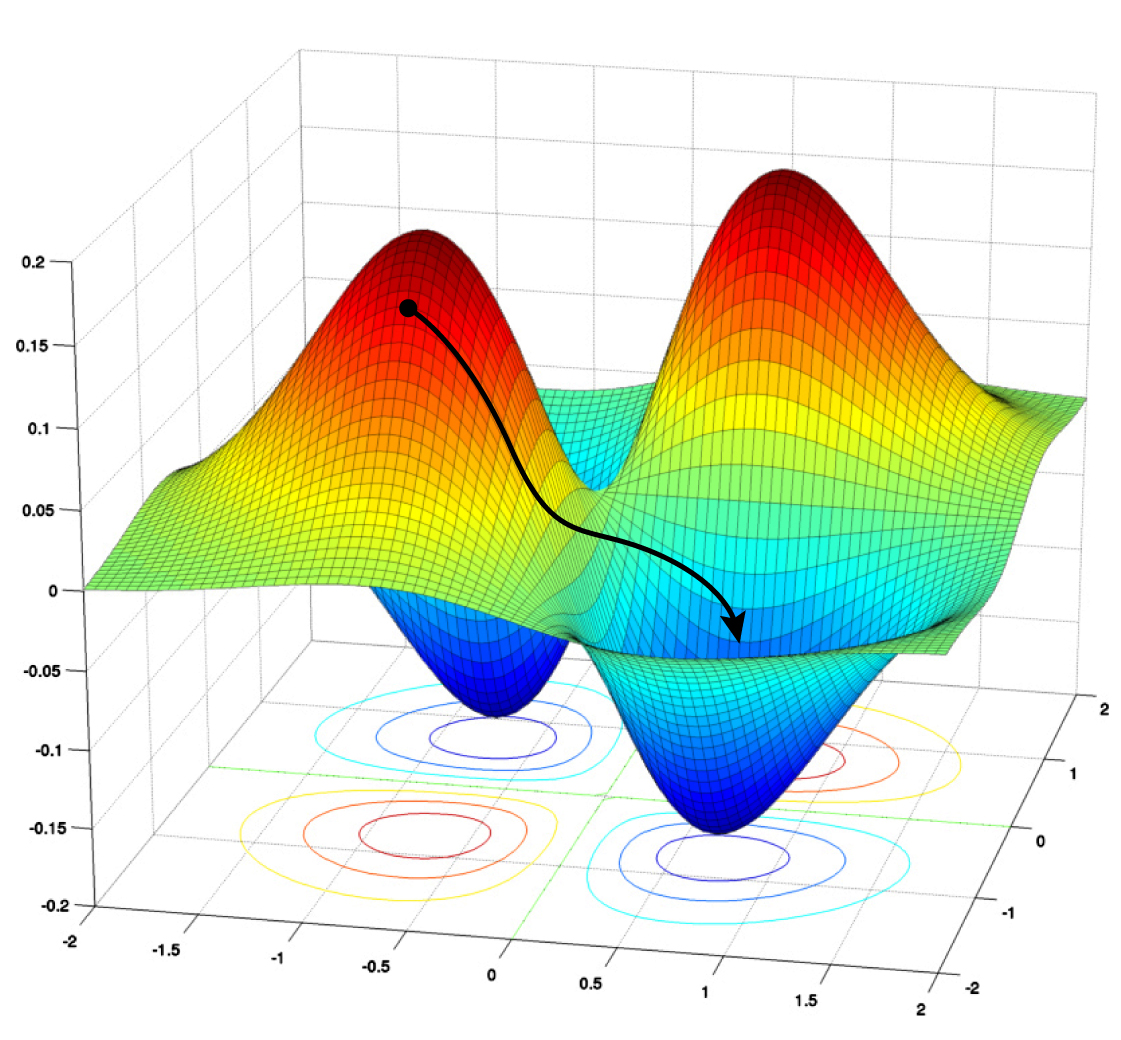
\includegraphics[width=\textwidth/2]{kapitel2/Gradient-descent.jpg}
    \caption{Gradient descent in a three-dimensional space. The graph represents the loss gradient and the black line shows a possible path that may be taken during gradient descent, which will eventually land in the minimum it is approaching\protect\footnotemark.}
    \label{fig:graddesc}
\end{figure}

\footnotetext{Image from \url{https://math.stackexchange.com/questions/406038/second-partial-derivative-test-question} (last visited on 2024-10-31) with modifications from \url{https://www.quantamagazine.org/researchers-build-ai-that-builds-ai-20220125/} (last visited on 2024-10-31)}

A more commonly used modern method is \ac{adam} \cite{Kingma.2015} or its derivatives like AdamW, which builds upon AdaGrad \cite{Duchi.2011} and RMSProp \cite{Tieleman.2012}.
Pseudocode for the \ac{adam} algorithm is shown in algorithm \ref{alg:adam}.
\ac{adam} utilizes two moment estimates, $m_t$ and $v_t$ which track the exponential moving averages of the gradient and the squared gradient respectively.
$\beta_1$ and $\beta_2$ are their respective exponential decay rates.
$m_t$ and $v_t$ are biased towards zero because they are initialized with it, which is why a bias-correction step is necessary for both.
$m_t$ and $v_t$ are both derived from $g_t$, which represents the gradient matrix of the model at step $t$, which could be once per sample, once per epoch, or once per batch.
An epoch is a full training pass of the entire dataset.
Data is sometimes grouped into so-called batches during training.
$\widehat{m}_t$ takes a role similarly to momentum.
Momentum is used to recognize if $g_t$ has a preferred direction by tracking the total average.
It can then accelerate movement in that direction, which is useful to skip over noisy gradients.
$\widehat{v}_t$ acts as variance detection and helps adjust the step size based on past gradient magnitude, allowing for large steps in a shallow gradient and small steps in steep gradients.
The weights are then updated, with $\alpha$ serving as a baseline step-size, $\widehat{m}_t$ deciding a direction and speed of the change, $\widehat{v}_t$ acting as a regulator based on the gradient and $\epsilon$ preventing division by zero. \cite{Kingma.2015}

\begin{algorithm}
    \centering
    \caption{The Adam optimizer update algorithm. $g^2_t$ is the elementwise square $g_t \odot g_t$. Kingma et al. recommend $\alpha = 0.0001$, $\beta_1 = 0.9$, $\beta_2 = 0.999$ and $\epsilon = 10^{-8}$ as default values. Algorithm taken from \cite{Kingma.2015}.}
    \begin{algorithmic}
    \Require $\alpha$: Stepsize
    \Require $\beta_1, \beta_2 \in [0,1)$: Exponential decay rates for the moment estimates
    \Require $f(\theta)$: Stochastic objective function with parameters $\theta$
    \Require $\theta_0$: Initial parameter vector

    \State $m_0 \leftarrow 0$ (Initialize 1\textsuperscript{st} moment vector)
    \State $v_0 \leftarrow 0$ (Initialize 2\textsuperscript{nd} moment vector)
    \State $t \leftarrow 0$ (Initialize timestep)

    \While{$\theta_t $ not converged}
        \State $t \leftarrow t+1$
        \State $g_t \leftarrow \nabla{\theta}f_t(\theta_{t-1})$ (Get gradients w.r.t stochastic objective at timestep $t$)
        \State $m_t \leftarrow \beta_1 \cdot m_{t-1} + (1 - \beta_1) \cdot g_t$ (Update biased first raw moment estimate)
        \State $v_t \leftarrow \beta_2 \cdot v_{t-1} + (1 - \beta_1) \cdot g^2_t$ (Update biased second raw moment estimate)
        \State $\widehat{m}_t \leftarrow m_t / (1 - \beta^t_1)$ (Compute bias-corrected first moment estimate)
        \State $\widehat{v}_t \leftarrow v_t / (1 - \beta^t_2)$ (Compute bias-corrected first moment estimate)
        \State $\theta_t \leftarrow \theta_{t-1} - \alpha \cdot \widehat{m}_t / (\sqrt{\widehat{v}_t} + \epsilon)$ (Update parameters)
    \EndWhile

    \State \Return $\theta_t$ (Resulting parameters)
    \end{algorithmic}
    \label{alg:adam}
\end{algorithm}


\subsection{Tokenization and Word Embeddings}
\label{sec:embeddings}
An important consideration in \ac{nlp} is how to feed textual data into models -- how can words be converted into a format that a model can understand?
In modern \ac{nlp}, there are two main components to this: \emph{tokenization} and \emph{word embeddings}.

Tokenization is the process of turning a text into an array of tokens using a tokenizer \cite{Jurafsky.2024,Nadkarni.2011}.
It is one of the first steps in the \ac{nlp} pipeline because models do not understand plain language string inputs, only numbers arranged into input vectors.
Tokens can be letter by letter, word for word, syllable by syllable, differentiating capital letters or not, treating special chararacters as unique tokens, among other possible groupings which are tokenizer-specific.
Tokenization is done with a vocabulary -- a mapping of known \enquote{text chunks} to their respective tokens.
Taking the example sentence \enquote{a token is a number.} and the tokenizer vocabulary \{' ' = 0, 'a' = 1, 'token' = 2, 'is' = 3, 'number' = 4, '.' = 5\}, then the resulting tokenized representation would be [1, 0, 2, 0, 3, 0, 1, 0, 4, 5].
Tokenization also includes \emph{padding} and \emph{truncation}.
Because models often have a fixed input size, any data that is inserted must be fitted to that size.
Padding adds dummy tokens to the end of the input if it is too short while truncation cuts any excess tokens if it is too long.

Embeddings are a bit more complicated.
A word embedding refers to a representation of the meaning behind a word, typically represented by a large-dimensional vector field where each dimension corresponds to some attribute of the word.
Words are often highly dependant on their context -- for example \enquote{He works at a bank}.
Which type of bank is being referred to?
Is the man is from Frankfurt, most likely a building.
If he is a fisherman, the river bank.
This is also language specific -- if the man is German, he may instead have a food truck at the park by the bench, as \enquote{Bank} can mean bench in German.
All of this information should be captured by an embedding to properly predict the most likely next word.

A well-known early embedding approach is Word2Vec, introduced by Mikolov et al. in 2013 \cite{Mikolov.2013b}.
It uses a vocabulary of around one million words and was trained on a text corpus of 6 billion words, the Google News corpus\footnote{\url{https://code.google.com/archive/p/word2vec/} (last visited on 2024-10-31)}.
The representations are trained with neural networks using stochastic gradient descent. Mikolov et al. further propose both continuous bag of words (CBOW) and Skip-gram as algorithms to predict a word from its context.
They find that in their representations, the relationships between words could be represented as algebraic operations, such as the following example: $vector("biggest") - vector("big") + vector("small")$ is roughly equivalent to $vector("smallest")$.
The same is applicable to the relationships between countries and capital cities being roughly the same vector or the famous $vector("King") - vector("Man") + vector("Woman") \approx vector("Queen")$ \cite{Mikolov.2013}.
Embeddings are often accompanied by a context size -- the number of words to look ahead and before to assess the context of each word individually.
A larger context size comes with more information, but also with more computational cost for the embedding.

In a modern system like the \ac{gpt}, the basis for ChatGPT, and the transformer architecture in general, which will be explained in further depth in section \ref{sec:transformer}, word embeddings are learned as part of the larger model alongside its other parameters \cite{Brown.2020}.
For comparison, the GPT-3 series uses word embeddings between 768 and 12.288 dimensions learned on 300 billion tokens \cite{Brown.2020} while the the Word2Vec paper examines between 50 and 1.000 dimensions for its tests \cite{Mikolov.2013b}.
Combining tokenization and embeddings is simple -- words are tokenized, the tokens are fed into the model and embeddings for the tokens are learned.
This may even allow new layers of context, especially if a word is split into multiple tokens.
The embedding for the token of \enquote{est} may contain the information that it is often a suffix and that, if at the end of a word, makes it a superlative, like the previously mentioned \enquote{biggest} and \enquote{smallest}.


\subsection{Transformers}
\label{sec:transformer}
Introduced by Google's research team in 2017 \cite{Vaswani.2017}, the transformer architecture has since become the standard for most \ac{llm} architectures.
Its defining characteristic and the paper's namesake is the self-attention mechanism, which will be explained later in this section.

A full transformer consists of one or more encoder blocks and one or more decoder blocks (introduced by \cite{Cho.2014}), as seen in figure \ref{fig:transformer}, but encoder-only (e.g. BERT \cite{Devlin.2019}) and decoder-only (e.g. GPT \cite{AlecRadfordKarthikNarasimhanTimSalimansIlyaSutskever.2018}) architectures have also become prevalent.

\begin{figure}[h]
    \centering
    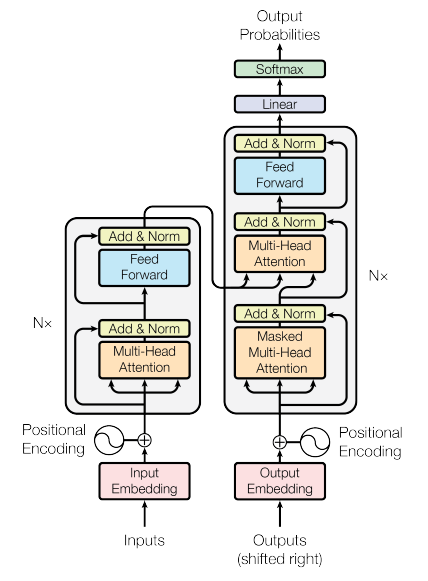
\includegraphics[width=\textwidth*2/3]{bilder/kapitel2/transformer.png}
    \caption{The full transformer architecture, consisting of embeddings, positional encoding and N encoder- and decoder blocks including attention heads and \acp{fnn}. Image taken from \cite{Vaswani.2017}.}
    \label{fig:transformer}
\end{figure}

The encoder turns an input sequence $(x_1, ..., x_n)$ into a sequence of continuous representations $z = (z_1, ..., z_n)$. The decoder generates a new output sequence $(y_1, ..., y_m)$ for a given input sequence $z$ \cite{Vaswani.2017, Cho.2014}.
More plainly, the encoder learns to create a hidden representations of a sequence of tokens and the decoder generates the most likely next token(s) to follow such a sequence.
Both blocks consist of the same components:

\paragraph{The Embedding Layer} turns the input tokens into their learned word embedding representations of size $d^{model}$ ($=512$ in the paper \cite{Vaswani.2017}).

\paragraph{The Positional Encoding} exists to add information to a token about its position within a given sequence.
These encodings have the same dimension as the embeddings, $d_{model}$, so they can be summed.
The original paper calculates the positional encoding as
\begin{equation}
    \begin{aligned}
        PE_{(pos,2i)} &= sin(pos/1000^{2i/d_{model}}) \text{ (even }i\text{)} \\
        PE_{(pos,2i+1)} &= cos(pos/1000^{2i/d_{model}}) \text{ (odd }i\text{)}
    \end{aligned}
\end{equation}
where $pos$ is the position of the token in the sequence and $i$ is the dimension of the positional encoding \cite{Vaswani.2017}.

\paragraph{The (Masked) Multi-Head Attention} is essentially a mechanism for the model to learn relationship between tokens in a sequence.
The goal of this mechanism is to calculate how closely a token is related to all other tokens.
In multi-head attention, multiple attention layers are used so that relationships can be established on different levels simultaneously, be that similar words, grammatical structure, word function, multi-token names, which noun a pronoun refers to and many more.
The original paper uses eight attention heads \cite{Vaswani.2017}.
Within the attention mechanism, a query, key and value vector are used to calculate the output with the equation
\begin{equation}
    \text{Attention}(Q,K,V)=\text{softmax}(\frac{QK^T}{\sqrt{d_k}})V
\end{equation}
where $d_k$ is the dimenion of $Q$ and $K$ \cite{Vaswani.2017}.
$Q$, $K$ and $V$ are derived from the input through learned projections.
A visualization of an attention output can be seen in figure \ref{fig:attention}.

\begin{figure}
    \centering
    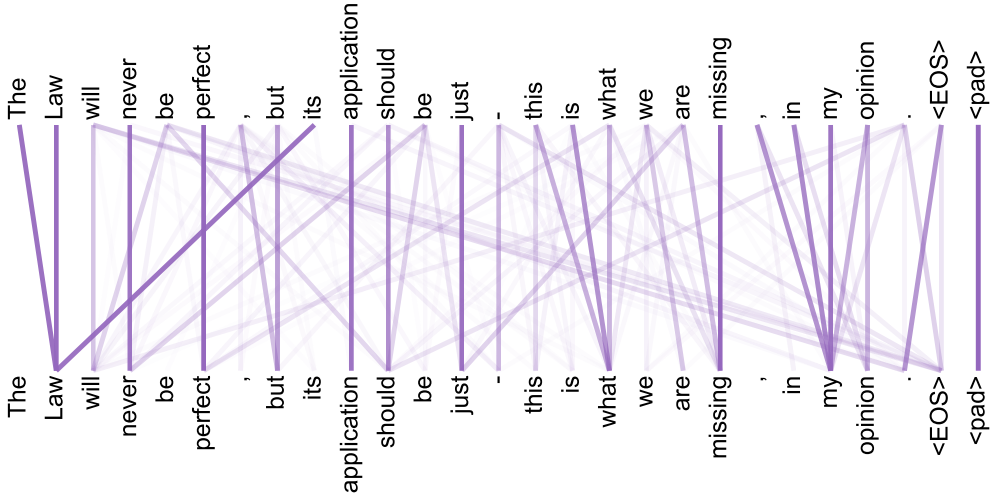
\includegraphics[width=\textwidth]{kapitel2/attention.png}
    \caption{A visualization of the output of one attention head. A darker purple means a stronger connection. For example, the word \enquote{its} strongly correlates to the word \enquote{Law}, as the former is a pronoun referring to the latter. Image taken from \cite{Vaswani.2017}.}
    \label{fig:attention}
\end{figure}

\paragraph{The Feedforward Neural Network} is, as explained in section \ref{sec:fnn}, a network of neurons grouped into layers that processes hidden representations of inputs through its layer configurations and weights learned with a training corpus.
\newline

For the original paper, the encoder layer consists of input embeddings, positional encoding, and N blocks of a multi-head attention layer followed by a feedforward layer.
These N blocks all have the exact same dimensions.
The original paper uses six heads \cite{Vaswani.2017}.
The decoder layer similarly consists of output embeddings, positional encoding, followed by N blocks of a masked multi-head attention layer, a multi-head attention layer and a feedforward block.
The outputs being shifted to the right, in combination with the masked attention, prevents the prediction for position $i$ to look ahead, instead only getting information from previous positions in the sequence.
These N blocks are also all the same, with the original paper having six \cite{Vaswani.2017}.
The outputs of the encoder layer feed into the second attention layer in the decoder block.
Finally, the outputs are run through a linear layer (a layer with a linear activation function) and a softmax layer to calculate the outputs.

The purpose of shifting the outputs right and using the masked multi-head attention layer is to limit the attention on words that come before the current token.
This is because the decoder layer calculates the probabilities for the next token in the sequence, meaning it does not have tokens following it and it can only look backwards for context.

One of the main advantages of the transformer is its high parallelizability during training, as opposed to recurrent models.
Being able to process multiple tokens simultaneously allows for much faster training, and is what enables transformers to be effectively trained on GPUs, which specialize in parallelized operations.
Because the transformer architecture has become so prevalent, when this thesis mentions \acp{lm} or \acp{llm}, it will refer to a transformer architecture unless otherwise specified.

\begin{comment}
\subsection{Code Synthesis}
\label{sec:codesynth}
(Probably don't need this section)
Code synthesis describes the generation of code syntax by a computer.

 PCFG and AST
 Code2Seq
 Latent Predictor Networks
 CodeBERT

In terms of \ac{nlp}, code is structured much differently from natural language on multiple levels.
It has a much more rigid structure that it must adhere to to work, has a much more limited vocabulary for anything other than user-given variable names (which are comparable to named entitites in regular \ac{nlp}), and it is not structured sequentially, but rather like a tree (called the \ac{ast}).
Words and punctuation can also different meanings in code and are much more strictly defined, losing much of their ambiguous context.
The word \enquote{if} would normally be followed by a pronoun and a verb in natural language, but by a condition statement in a bracket in code.
With code, much closer attention needs to be put on syntax.
If a natural \acl{lm} forgets to generate a comma, the sentence is typically still legible.
If a code synthesis model forgets a bracket, the code has an error and cannot run.
Further, code needs to be functionally correct, meaning it has to produce the desired output.
Metrics like the BLEU score break down in assessing code generation, because code that looks similar does not always behave the same, and code that does not look similar can behave identically.
\end{comment}



\subsection{Parameter-Efficient Fine-Tuning}
\label{sec:peft}

As \acp{lm} become more and more complex, fine-tuning them for specific purposes becomes a daunting task.
\acp{llm} especially have been trained on state-of-the-art hardware for months and have billions of parameters.
Fine-tuning all parameters of such a model requires an immense amount of processing power, memory and storage space.
\ac{peft} is a field of study to reduce this cost by exploring alternative ways of fine-tuning other than simple full-parameter fine-tuning.


\subsubsection{LoRA}
\label{sec:lora}

\begin{figure}
    \centering
    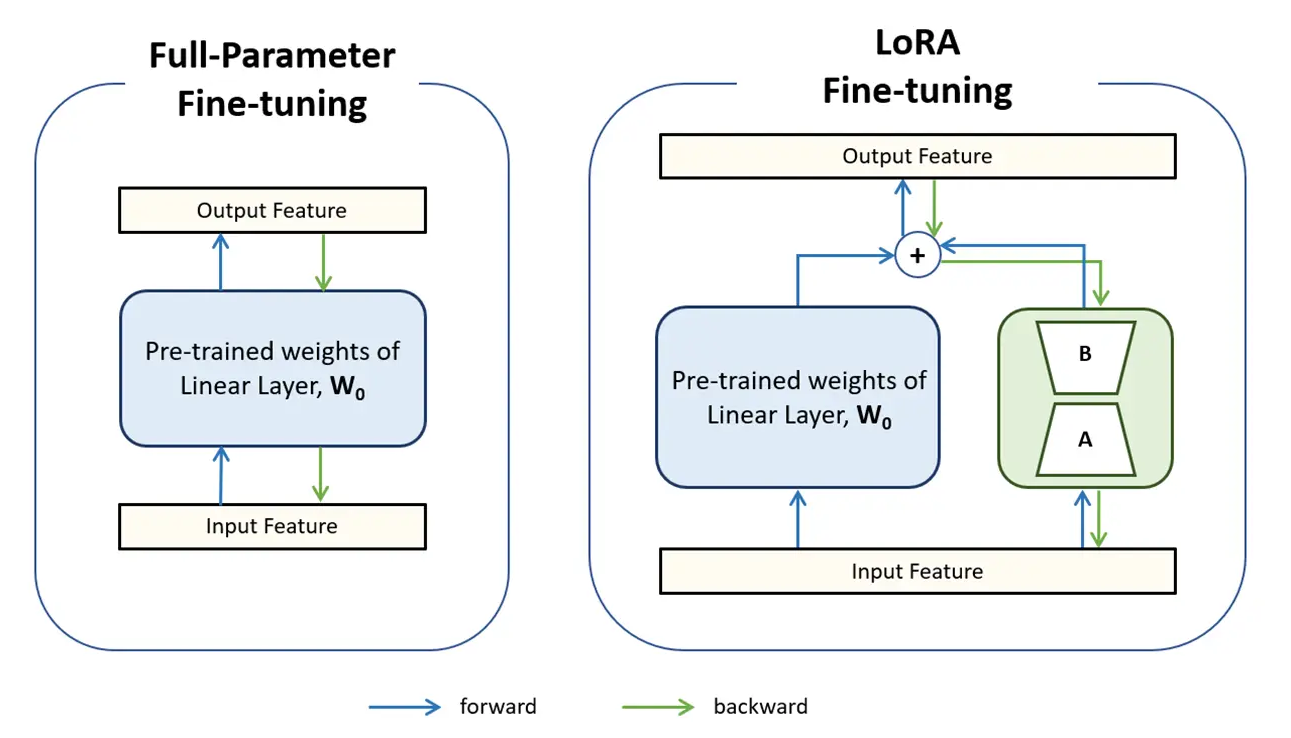
\includegraphics[width=\textwidth]{bilder/kapitel2/lora.png}
    \caption{Full-parameter fine-tuning and \ac{lora} fine-tuning. \ac{lora} adds the new matrices A and B which are trained rather than the pre-trained weights W$_0$\protect\footnotemark.}
    \label{fig:lora}
\end{figure}
\footnotetext{Image taken from \url{https://developer.habana.ai/blog/fine-tuning-llama2-70b-with-deepspeed-zero-3-and-low-rank-adaptation-lora-on-intel-gaudi2-ai-accelerator} (last visited on 2024-10-31)}

\Ac{lora} is a popular method to efficiently fine-tune \acp{lm}.
Introduced by Microsoft's Hu et al. in 2021 \cite{Hu.2022}, \ac{lora} does not directly train and alter the weights of a model.
Instead, it freezes the pre-trained weights and introduces new weights to train into the model.
This has a few advantages: Training the new weights is much less computationally intense and adding new weights lets the model keep all of its old weights intact.

It allows the training of multiple downstream tasks from a single model easily by simply saving the newly learned weights, which also saves massively on storage space the larger the model is, and it prevents \emph{catastrophic forgetting}, where weights are altered to such an extent that previously acquired knowledge is lost.
\ac{lora} configurations built onto the same model can even be swapped out at runtime, allowing a much more performant model for multiple specific tasks at reduced storage and processing costs.
\ac{lora} weights are saved as two low-ranking matrices, representing each of the dimensions of the model's weights which they aim to fine-tune \cite{Hu.2022}.
This is done because Hu et al. assert that a model's weight matrices do not need to be fully adjusted during training, and that a smaller subset of weight changes can capture the desired change equally well.
In this context, rank refers to the number of linearly independant rows or columns, and Hu et al. argue that the ranks of weight matrices are often smaller than their actual dimensions, meaning they carry superfluous information.
Given a weight matrix of a size $d \times k$ and a chosen rank $r$ between 1 and $\min(d,k)$, training with \ac{lora} would use two matrices of sizes $d \times r$ and $r \times k$, then multiply them together to get the original matrix size.
This can be expressed as

\begin{equation}
    h = W_0x + \Delta Wx = W_0x + BAx
\end{equation}

where $h$ is the fine-tuned weight matrix, $W_0 \in \mathbb{R}^{d\times k}$ is the pre-trained weight matrix and $B \in \mathbb{R}^{d\times r}, A \in \mathbb{R}^{r\times k}$ are the low-rank matrices which produce $\Delta W$ when multiplied \cite{Hu.2022}.

One might expect that finding an appropriate size for $r$ which balances performance and accuracy depends on the task.
A smaller $r$ could mean better performance as the size of the matrix is decreased, but in turn can also lead to lower accuracy as detail is lost if the chosen rank is lower than the \enquote{optimal rank} for the respective weights.
However, as the original paper finds, very small ranks, even a rank of one, are sufficient for fine-tuning in many cases, and applying \ac{lora} to more weight matrices with a lower rank is preferable to applying it to fewer matrices with a larger one \cite{Hu.2022}.

\subsubsection{QLoRA}
\label{sec:qlora}
Dettmers et al. introduced \ac{qlora} in 2023 \cite{Dettmers.2023}, building upon the low-rank approach introduced with \ac{lora}.
Quantization refers to the act of transforming a piece of information or data into a representation that holds less information.
In the case of computers, this means transforming higher-bit representations into lower-bit representation.
\ac{qlora} contains three primary contributions: NF4, double quantization and paged optimizers.
NF4 refers to 4-bit NormalFloat, a newly introduced datatype that builds on quantile quantization.
It works as follows:
It estimates $2^l+1$ quantiles from the input to create a $k$-bit quantile quantization data type, normalizes them to $[-1,1]$.
It also quantizes an input weight tensor, also normalizing it to $[-1,1]$ through absolute maximum rescaling and with the help of quantization constants.
Dettmers. et al. posit that weight tensors often follow a zero-centered normal distribution with a standard deviation $\sigma$, which allows this normalization into a fixed distribution.
Quantiles are estimated according to

\begin{equation}
    q_i = \frac{1}{2} \left( Q_{\mathrm{x}} \left( \frac{i}{2^k+1} \right) + Q_{\mathrm{x}} \left( \frac{i+1}{2^k+1} \right) \right)
\end{equation}

where $Q_{\mathrm{x}}(\cdot)$ is the quantile function of the standard normal distribution $N(0,1)$ \cite{Dettmers.2023}.
Once the input and data types are normalized, the inputs can be mapped to the closest quantized representation.
In order to represent zero, two symmetric quantile sets are estimated, one for a positive range (of size $2^{k-1}+1$) and one for a negative range (of size $2^{k-1}$).
One of the zeroes is discarded and the two sets are combined into an asymmetric set with a single zero at its center.
The resulting information-theoretically optimal data type is called $k$-bit NormalFloat (NF$k$), with \ac{qlora} using $k=4$ \cite{Dettmers.2023}.

Double quantization takes the quantization constants $c_2$\textsuperscript{FP32} of the first quantization and quantizes them to save even more memory.
It transforms them into $c_2$\textsuperscript{FP8} with its own set of quantization constants $c_1$\textsuperscript{FP32}.
The superset text refers to the bit size or data type of the respective value, in this case 8-bit or 32-bit floating point.
Dettmers et al. calculate a reduction of 0.5 bits to 0.127 bits per parameter on average for a blocksize of 64 and 32-bit floating point constants \cite{Dettmers.2023}.
Paged optimizers utilize NVIDIAs unified memory to offload processing from the GPU to the CPU when the GPU runs out of memory.
Combining everything, Dettmers et al. define the output for a single linear layer of a quantized base model with one \ac{lora} adapter using \ac{qlora} as

\begin{equation}
    \mathbf{Y}^{\text{BF16}} = \mathbf{X}^{\text{BF16}} \text{doubleDequant} (c_1^{\text{FP32}},c_2^{\text{k-bit}},\textbf{W}^{\text{NF4}}) + \mathbf{X}^{\text{BF16}} \mathbf{L}_1^{\text{BF16}} \mathbf{L}_2^{\text{BF16}}
\end{equation}
with
\begin{equation}
    \text{doubleDequant} (c_1^{\text{FP32}},c_2^{\text{k-bit}},\textbf{W}^{\text{k-bit}}) = \text{dequant}(\text{dequant}(c_1^{\text{FP32}},c_2^{\text{k-bit}}), \textbf{W}^{\text{4-bit}}) = \textbf{W}^{\text{BF16}}
\end{equation}
where $\mathbf{X}$ is the input, $\mathbf{W}$ are the quantized weights, $\mathbf{Y}$ is the output, $c_1$ and $c_2$ are the quantization constants and $L_1$ and $L_2$ are equivalent to the \ac{lora} matrices $A$ and $B$ explained in section \ref{sec:lora} \cite{Dettmers.2023}.

During evaluation, they establish that 4-bit \ac{qlora} matches 16-bit full finetuning in performance on benchmarks like GLUE \cite{Wang.2018} and T$k$-Instruct \cite{Wang.2022}.
They note that \ac{qlora} reduces the average memory requirements of finetuning a 65 B parameter model from over 780 GB GPU memory to under 48 GB without affecting the runtime or model performance when compared to full 16-bit finetuning.
They also finetune the Guanaco 65 B model on OASST1 using \ac{qlora}, producing the best open-source chatbot of its time, comparable in performance to ChatGPT on the Vicuna benchmark \cite{Chiang.2023}.
Their thesis concludes that \ac{qlora} makes the creation of performant models much more accessible because of the reduced cost for training models \cite{Dettmers.2023}.


\section{Evaluation Metrics}
\label{sec:metrics}

Because the development of code synthesis \acp{lm} has become increasingly popular, many metrics and frameworks for testing their coding ability have been developed.
This section will introduce some of these metrics and frameworks, which will be used to judge the coding ability of the TinyFuncCoder models introduced by this thesis.
Many of the presented metrics are part of the Bigcode Evaluation Harness \cite{BenAllal.2022}, a collection of metrics for assessing code synthesis ability of \acp{lm}.
The metrics of the BigCode Evaluation Harness that did not get their own sections were not considered for the following reasons:
\begin{itemize}
    \item InstructHumanEval\footnote{\url{https://huggingface.co/datasets/codeparrot/instructhumaneval} (last visited on 2024-10-31)} reformats the HumanEval prompt and is incompatible with the prompt template for TinyFuncCoder.
    \item APPS \cite{Hendrycks.2021} consists of 10.000 Python problems. Python is overrepresented in the evaluation metrics, as discussed in chapter \ref{chap:discussion}, and evaluating on 10.000 problems is not feasible within the time constraints of the thesis.
    \item Recode \cite{Wang.2022} perturbs HumanEval problems, effectively just increasing the amount of problems close to identical to HumanEval the model has to solve.
    \item PAL \cite{Gao.2023} is not compatible with TinyFuncCoder's prompt template.
    \item CodeXGLUE \cite{Lu.2021} is a code to text task, which TinyFuncCoder is not trained for.
    \item CoNaLa (Python) \cite{Yin.2018} and Concode (Java) \cite{Iyer.2018} use BLEU, which is deemed an unsuitable metric for code synthesis evaluation \cite{Chen.2021,Luo.2024}.
    \item Java complexity prediction \cite{Jeon.2023}, Java code equivalence prediction \cite{Svajlenko.2014,Wang.2020} and C code defect prediction \cite{Zhou.2019} are downstream classification tasks, which TinyFuncCoder is not trained for.
    \item SantaCoder-FIM \cite{Allal.2023} is an infilling task, which TinyFuncCoder is not trained for.
    \item Mercury \cite{Du.2024} evaluates code efficiency, which TinyFuncCoder is not capable enough to benefit from analyzing.
\end{itemize}

\subsection{HumanEval}
\label{sec:humaneval}
In their 2021 paper, Chen et al. introduce the Codex \ac{llm} and -- more importantly for this thesis -- the HumanEval evaluation framework \cite{Chen.2021}.
The HumanEval framework is a set of programming challenges with associated unit tests.
It judges the coding ability of \acp{lm} by prompting them with a challenge and then seeing if the resulting code passes its unit tests.
This method of checking functional correctness differs from previously used \ac{nlp} metrics like the BLEU score \cite{Papineni.2001}, which matches or fuzzy matches the output to an existing, expected result.
Because the BLEU score has been found as inefficient \cite{Chen.2021,Luo.2024}, Chen et al. use the pass@$k$ metric \cite{Kulal.2019}.
They deviate from the original definition where $k$ samples are generated and pass@$k$ is defined by $\frac{c}{k}$, where $c$ is the number of samples that pass all tests.
Instead, they give a mathematically less biased definition that reduces the otherwise high variance:
\begin{equation}
    \text{pass@}k := \underset{\text{Problems}}{\mathbb{E}} \left[ 1 - \frac{ \left( \begin{array}{c} n-c \\ k \end{array} \right) }{ \left( \begin{array}{c} n \\ k \end{array} \right) } \right]
    \label{eq:passk}
\end{equation}
where $n \geq k$ samples are generated and $c \leq n$ correct samples are produced \cite{Chen.2021}.
Commonly, either pass@1, pass@10 or pass@100 are used for evaluation.
Pass@$k$ has become the metric of choice for evaluating code synthesis ability on most benchmarks.

HumanEval consists of 164 hand-written challenges with an average of 7.7 tests per problem.
The problems include a function signature, docstring, the tests and a body.
They are written exclusively in Python, meaning it can only evaluate how good the Python code a model can synthesise is \cite{Chen.2021}.
As the paper focuses mainly on Codex, not much detail is given as to how the questions were written and decided on. % page 25
It is simply stated that they assess \enquote{language comprehension, reasoning, algorithms, and simple mathematics} \cite{Chen.2021}.
The appendix adds some elaboration and goes into detail about the attributes that were focused on when creating the dataset, but still does not give a proper explanation for its creation.

When evaluating on HumanEval, Chen et al. find that the temperature used for generation should be chosen in relation to $k$ when evaluating on the pass@$k$ metric.
The temperature regulates the amount of randomness in the generation, with a temperature of zero always giving the same result, and a temperature of one varying wildly in output.
They specify that $k$=1 should have a temperature of around 0.2 when generating and $k$=100 a temperature of around 0.8.
On their largest model with $10^{10}$ parameters, they achieve a pass@1 of around 30\% and a pass@100 of around 70\% using the previously given temperatures.

\subsection{MBPP}
\label{sec:mbpp}
\ac{mbpp} was introduced by Odena et al. of Google Research \cite{Odena.2021} alongside MathQA-Python.
It consists of 974 programming tasks intended to be solvable by entry-level programmers.
They are given as a natural language prompt with three example calls to the function with an expected result in the form of assertions the function should pass.
Similarly to HumanEval, these tasks are all given exclusively in Python.

When evaluating code synthesis ability, Odena et al. note that larger models perform better, with the largest at 137 B parameters synthesising solutions for 59.6\% of problems with few-shot learning.
They further note that fine-tuning on their set of only 374 problems improves performance by around ten percent across all models.

To create the dataset, crowdworkers with knowledge of Python were asked to write basic Python problems, a corresponding solution, and three test cases for the given function.
A hand-filtered subset of this dataset was also created.
This resulted in a dataset of 476 problems for which the authors ensure a standard Python signature, an unambiguous description and accurate test cases.
Both the full set and the edited set were used in their testing.


\subsection{EvalPlus}
\label{sec:evalplus}

\begin{figure}
    \centering
    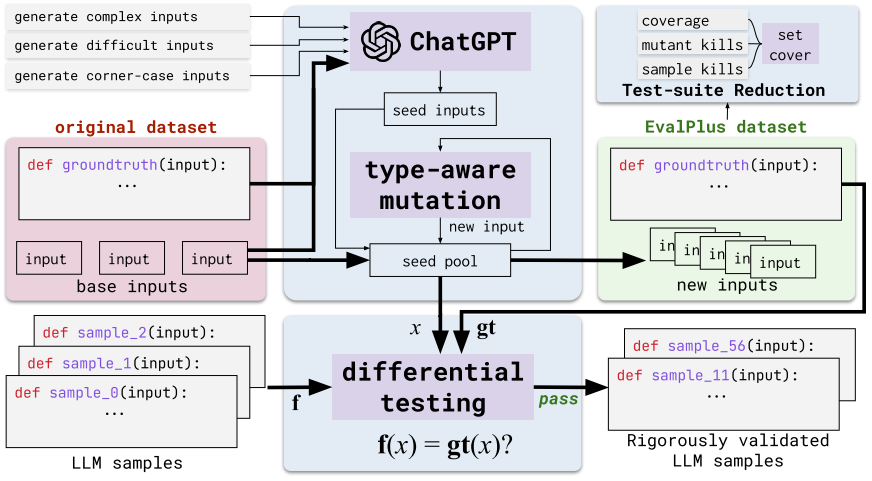
\includegraphics[width=\textwidth]{bilder/kapitel2/evalplus.png}
    \caption{Generation of new test cases using the EvalPlus framework. Image taken from \cite{Liu.2024}.}
    \label{fig:evalplus}
\end{figure}

The EvalPlus framework, introduced by Liu et al. \cite{Liu.2024}, aims to improve upon other code synthesis assessment metrics by expanding their test suites with the help of \acp{llm}.
Their paper mainly showcases this framework when applied to HumanEval, creating HumanEval+, but they have since also created MBPP+ with it.
As it only expands the test coverage, the problems are identical to the base versions but the generated results are checked more thoroughly, and by extension so is model performance on the pass@$k$ metric.

Their main points of criticism of coding metrics are that problems are given with imprecise descriptions and with an average of less than ten tests per problem.
They argue that imprecise descriptions fail to fully clarify the expected behaviours of the generated code and that a lack of proper testing leads to many false positives because edge cases are not properly covered.

The EvalPlus framework generates new test cases as follows:
First, it takes the original ground-truth implementations and one of its three test cases as an input. Together with a prompt (one of \enquote{generate [complex|difficult|corner-case] inputs}), ChatGPT is queried to generate seed inputs, only filtering out results which do not adhere to the format expected by the ground-truth implementation.

Next, type-aware input mutation \cite{Winterer.2020} is performed on the seed inputs. This means altering the provided test cases by altering the given inputs in some way. Inputs are altered differently depending on their data type, hence type-aware. The applied mutations are listed in table \ref{tab:mutation}.
%\renewcommand{\arraystretch}{1.2}

\begin{table}
    \centering
    \small
    \caption{Mutations used by the EvalPlus framework to alter inputs. \texttt{Mutate} refers to a recursive function to alter an inner type (for example, the int mutation can be applied to a random subset of a list of ints). Table taken from \cite{Liu.2024}.}
    \begin{tabular}{ll|ll}
        \hline
        Type & Mutation & Type & Mutation\\
        \hline
        \texttt{int} | \texttt{float} & Returns $x\pm1$ &
        \texttt{List} & $\left\{\begin{tabular}{@{\ }l@{}}
            Remove/repeat a random item $x[i]$ \\ Insert/replace $x[i]$ with \texttt{Mutate($x[i]$)}\end{tabular}\right.$ \\
        \texttt{bool} & Returns a random boolean &
        \texttt{Tuple} & Returns \texttt{Tuple(Mutate(List($x$)))} \\
        \texttt{NoneType} & Returns \texttt{None} &
        \texttt{Set} & Returns \texttt{Set(Mutate(List($x$)))}\\
        \texttt{str} & $\left\{\begin{tabular}{@{\ }l@{}}
            Remove a sub-string $s$ \\ Repeat a sub-string $s$  \\ Replace $s$ with \texttt{Mutate}($s$)\end{tabular}\right.$ &
    \texttt{Dict} & $\left\{\begin{tabular}{@{\ }l@{}}
            Remove a key-value pair $k\rightarrow v$ \\ Update $k\rightarrow v$ to $k\rightarrow$ \texttt{Mutate($v$)}  \\ Insert \texttt{Mutate($k$)$\rightarrow$Mutate($v$)}
    \end{tabular}\right.$ \\
        \hline
    \end{tabular}
    \label{tab:mutation}
\end{table}

Finally, a smaller subset called HumanEval+-Mini is created by reducing the HumanEval+ set by a factor of 47, focusing on keeping a similar branch coverage and pruning tests through mutation testing and \ac{llm} sample killings.
A full overview of this process is shown in figure \ref{fig:evalplus}.
To ensure that their tests work, they follow the principle of design by contract \cite{Meyer.1992}, which they implement through assert statements to ensure well-formed inputs.

Liu et al. also tested HumanEval+ with over 26 \acp{llm} and various temperature settings.
They find that performance on the pass@$k$ metric (\ref{eq:passk}) sank across the board in all tests, with drops of 19.3\%, 24.9\% and 28.9\% for $k$ = 1, 10 and 100 respectively.
HumanEval+-Mini achieves similar results, with the drop in performance being slightly less than with the full suite.
They also found that around 11\% of the original ground-truth implementations were incorrect and reimplemented them.

\subsection{MultiPL-E}
\label{sec:multiple}
MultiPL-E, introduced by Cassano et al. \cite{Cassano.2023}, extends HumanEval and \ac{mbpp} to 18 programming languages, the first massively multilingual code generation benchmark according to the paper.
It does this by writing a compiler for each language that translates the function head and tests from Python to the language.
Each compiler is around 200 lines of code.
Python-specific description vocabulary is also altered manually, and typing discrepancies between languages are taken into consideration, such as translating Python tuples and lists into JavaScript arrays.
Having a compiler for each language also makes the benchmark easily extendible.

When testing MultiPL-E with Codex \cite{Chen.2021}, CodeGen \cite{Nijkamp.2022} and InCoder \cite{Fried.2023}, Cassano et al. replicate the findings on Python performance from these three models and achieve surprisingly good results on most languages, even those that were not included in the original training sets for the models.
They also find that performance on JavaScript and TypeScript problems is similarly high to, and sometimes exceeds, performance on Python problems.

\subsection{HumanEvalPack}
\label{sec:octopack}
Similarly to MultiPL-E, the HumanEvalPack, introduced by Muennighoff et al. \cite{Muennighoff.2024}, aims to expand HumanEval by multiple languages.
Rather than the 18 of MultiPL-E, HumanEvalPack extends to six languages and does not include MBPP.
Like most other problem packs, it evaluates on the pass@$k$ metric and features three sets of problems: HumanEvalFix for repairing buggy code, HumanEvalExplain for explaining given code and then generating a solution this explanation, and HumanEvalSynthesize for generating new code (corresponding to the original HumanEval).
For HumanEvalFix, a bug was manually added to each of the 164 HumanEval problems for each of the six languages for the model to solve.
This gives an equivalent size of $164\cdot6$ for all three sections, or a total of 2952.
All the new content of the HumanEvalPack is created by humans, unlike MultiPL-E, which compiles problems to new languages or EvalPlus, which generates new problems through mutation.


\subsection{DS-1000}
\label{sec:ds1000}
DS-1000 is a set of 1000 data science problems to evluate code synthesis performance.
It was introduced by Lai et al. \cite{Lai.2023}.
The problems are all given in Python, like MBPP and HumanEval, and span seven Python libraries: NumPy\footnote{\url{https://numpy.org/} (last visited on 2024-10-31)}, Pandas\footnote{\url{https://pandas.pydata.org/} (last visited on 2024-10-31)}, TensorFlow\footnote{\url{https://www.tensorflow.org/} (last visited on 2024-10-31)}, PyTorch\footnote{\url{https://pytorch.org/} (last visited on 2024-10-31)},
SciPy\footnote{\url{https://scipy.org/} (last visited on 2024-10-31)}, Scikit-learn\footnote{\url{https://scikit-learn.org/stable/} (last visited on 2024-10-31)} and Matplotlib\footnote{\url{https://matplotlib.org/} (last visited on 2024-10-31)}.
The problems in DS-1000 are collected from StackOverflow.
They were then manually curated and altered to adhere to three principles:
First, problems that are diverse in form and content, rather than highly structured, were chosen to better reflect real-world applications.
Second, five of the paper's authors adapted these natural problems by writing new code, adapting them to be more unambiguous, executable and testable, and writing tests for them.
Third, to prevent models from simply memorizing solutions from StackOverflow, they took active measures to perturb each problem.
Perturbations include paraphrasing a problem and altering semantic components \cite{Lai.2023}.
DS-1000 presents the problems in an infilling context, though many models lack this feature and can only generate left-to-right, meaning generating new tokens at the end of a sequence, rather than in the middle.
To address this, they offer a prompt to reformat the questions for left-to-right models, while acknowledging that these will still lack behind models with infilling capabilities.

Models from three families were also tested on DS-1000, with the best results coming from codex-davinci-002 (from the Codex family which was introduced alongside HumanEval \cite{Chen.2021}) at a pass@1 of 43.3\% when infilling and 39.2\% when generating left-to-right.
This leaves much room for improvement, with even the current best model, Claude 3.5 Sonnet, achieving a pass@1 of 54.3\%.
Many models have improved on codex-002 however, with it being in 29th place on the DS-1000 leaderboard\footnote{\url{https://ds1000-code-gen.github.io/model_DS1000.html} (last visited on 2024-10-31)}.


\subsection{LeetCode Contest Benchmark}
\label{sec:leetcode}
LeetCode\footnote{\url{https://leetcode.com/} (last visited on 2024-10-31)} is a website offering coding challenges for programmers to test and expand their skills in various categories and languages, with some of these being notoriously difficult.
It also offers code interview crash courses.
In their paper introducing DeepSeek-Coder, Guo et al. \cite{Guo.2024} also introduce the LeetCode Contest Benchmark\footnote{\url{https://github.com/deepseek-ai/DeepSeek-Coder/tree/main/Evaluation/LeetCode} (last visited on 2024-10-31)}, a collection of 180 LeetCode Contest challenges from July 2023 to January 2024, with 100 test cases per challenge.
These problems are formatted in the same way as HumanEval problems and are also only given in Python.
They gather these challenges to further evaluate DeepSeek-Coder, choosing 180 challenges that at the time of the papers release would not have appeared in their training data.
This is the only benchmark mentioned that is not featured in Bigcode's evaluation harness.

When evaluating model performance, their 6.7 B parameter model achieves a pass@1 of 19.4\% with the 33 B version achieving 27.8\%.
They further note that \ac{cot} prompting improved model performance on this benchmark, especially with more challenging problems.

\section{The Stack Dataset}
\label{sec:thestack}

Bigcode's The Stack \cite{Kocetkov.2023} is a 6.4 TB dataset encompassing permissively licensed GitHub files in 358 programming languages (the paper lists 3.1 TB with 30 languages, but the set has since expanded).
It is part of the BigCode project\footnote{\url{https://www.bigcode-project.org/} (last visited on 2024-10-31)}, a scientific collaboration to openly and transparently develop and share results in the code synthesis field.

There are various versions of The Stack\footnote{\url{https://huggingface.co/datasets/bigcode/the-stack} (last visited on 2024-10-31)}, including The Stack v2\footnote{\url{https://huggingface.co/datasets/bigcode/the-stack-v2} (last visited on 2024-10-31)} at 67.5 TB, as well as near-deduplicated versions\footnote{\url{https://huggingface.co/datasets/bigcode/the-stack-dedup}}\footnote{\url{https://huggingface.co/datasets/bigcode/the-stack-v2-dedup} (last visited on 2024-10-31)} of both.
Further, there is The Stack smol\footnote{\url{https://huggingface.co/datasets/bigcode/the-stack-smol} (last visited on 2024-10-31)}, a scaled-down version with 10.000 randomly sampled files per language, totalling 2.6 GB of data.

This thesis will work with the original The Stack's 3 TB deduplicated version.
The Stack v2 currently does not include the code as a string, for which the original has the \enquote{content} column, and the deduplicated version is recommended for training by the authors.
The Stack smol was used in preparation of the codebase for this thesis before The Stack was used for dataset creation.

The Stack dataset has the following data fields, as explained on huggingface:
\begin{itemize}
    \item \texttt{content} (\texttt{string}): the content of the file.
    \item \texttt{size} (\texttt{integer}): size of the uncompressed file.
    \item \texttt{lang} (\texttt{string}): the programming language.
    \item \texttt{ext} (\texttt{string}): file extension
    \item \texttt{avg\_line\_length} (\texttt{float}): the average line-length of the file.
    \item \texttt{max\_line\_length} (\texttt{integer}): the maximum line-length of the file.
    \item \texttt{alphanum\_fraction} (\texttt{float}): the fraction of characters in the file that are alphabetical or numerical characters.
    \item \texttt{hexsha} (\texttt{string}): unique git hash of file
    \item \texttt{max\_\{stars|forks|issues\}\_repo\_path} (\texttt{string}): path to file in repo containing this file with maximum number of \{stars|forks|issues\}
    \item \texttt{max\_\{stars|forks|issues\}\_repo\_name} (\texttt{string}): name of repo containing this file with maximum number of \{stars|forks|issues\}
    \item \texttt{max\_\{stars|forks|issues\}\_repo\_head\_hexsha} (\texttt{string}): hexsha of repository head
    \item \texttt{max\_\{stars|forks|issues\}\_repo\_licenses} (\texttt{string}): licenses in repository
    \item \texttt{max\_\{stars|forks|issues\}\_count} (\texttt{integer}): number of \{stars|forks|issues\} in repository
    \item \texttt{max\_\{stars|forks|issues\}\_repo\_\{stars|forks|issues\}\_min\_datetime} \\(\texttt{string}): first timestamp of a \{stars|forks|issues\} event
    \item \texttt{max\_\{stars|forks|issues\}\_repo\_\{stars|forks|issues\}\_max\_datetime} \\(\texttt{string}): last timestamp of a \{stars|forks|issues\} event
\end{itemize}
Of these, \texttt{content}, \texttt{lang}, \texttt{hexsha} and \texttt{max\_stars\_count} are used in this thesis, as further explained in section \ref{sec:data}.

The stack was created by first gathering a list of 220.92 M unique, active GitHub repository names from GHArchive\footnote{\url{http://www.gharchive.org/} (last visited on 2024-10-31)}, of which 137.36 M were succesfully downloaded.
Of the files contained in the repositories, binary files and files exceeding 1 MB are removed, resulting in 5.28 B files in total.
Next, the files were checked for their license using GHArchive and the go-license-detector\footnote{\url{https://github.com/src-d/go-license-detector} (last visited on 2024-10-31)} and only files with a permissive license were kept.
These files are then deduplicated \cite{He.2010} and near-deduplicated, removing all files that are copies or mostly overlapping, keeping a total remained of 3.1 TB of data \cite{Kocetkov.2023}.
Note that these numbers are from the time of the paper's release and the dataset has since grown.

A further filtered Python subset of The Stack was also used to train a 350 M parameter decoder-only transformer from scratch, achieving middling results with a pass@1 of 13.94 and pass@100 of 37.00 on HumanEval, and pass@1 of 15.94 and pass@100 of 54.69 on MBPP, but outperforming the similarly-sized Codex \cite{Chen.2021} and CodeGen \cite{Nijkamp.2022} \cite{Kocetkov.2023}.
How The Stack is filtered into TinyFuncData in this thesis is explained in section \ref{sec:data}.


\section{Base Models}
\label{sec:basemodels}

This section will introduce the base models that were considered for fine-tuning to create the TinyFuncCoder series.
It will explore possible options and present their up- and downsides.

\subsection{TinyLlama}
\label{sec:tinyllama}

TinyLlama\footnote{\url{https://huggingface.co/TinyLlama/TinyLlama-1.1B-Chat-v1.0} (last visited on 2024-10-31)} is a 1.1 B parameter model pre-trained on both natural language through SlimPajama \cite{Soboleva.2023} and code through Starcoderdata \cite{Li.2023b} at a ratio of about 7:3.
It was developed by Zhang et al. \cite{Zhang.2024} as a response to \ac{nlp} research focusing on increasingly larger models, aiming to show that small models can also achieve solid performance.
To achieve this, they pre-train a decoder-only transformer architecture on almost 3 T tokens -- 950 B tokens for three epochs.
The idea behind TinyLlama -- to squeeze as much performance as possible out of a small model -- makes it an obvious pick as a base model for TinyFuncCoder.
What makes it even more suited as a choice is that it is entirely open-source and advertises itself as an improvement in accessibility for \ac{lm} research and usage.

As stated in section \ref{sec:motivation}, being pretrained on Starcoderdata could be beneficial, but it could also be detrimental.
Having previous training on code could strengthen the new information injected during training, acting as a solid baseline to expand upon.
Because TinyFuncCoder aims to be very restrictive in its possible outputs however, prior code knowledge could also lead to unexpected behaviour and undesired answer formats.
When testing on HumanEval, TinyLlama achieves a score of 9.15.
It is unspecified for which metric, but a reasonable assumption is pass@1, placing it between Codex-85M and Codex-300M \cite{Chen.2021}.
The best Codex model, Codex-12B, achieves a pass@1 of 28.81\%.

During the writing of this thesis, a newer version of TinyLlama, TinyLlama v1.1\footnote{\url{https://huggingface.co/TinyLlama/TinyLlama_v1.1} (last visited on 2024-10-31)} was released.
It is split into three models -- a base version trained and fine-tuned only on SlimPajama, a math and code version fine-tuned on Starcoderdata and Proofpile\footnote{\url{https://huggingface.co/datasets/hoskinson-center/proof-pile} (last visited on 2024-10-31)}, and a Chinese version fine-tuned on Skypile \cite{Wei.2023}.


\subsection{Phi}
\label{sec:phi}
The Phi models\footnote{\url{https://huggingface.co/collections/microsoft/phi-3-6626e15e9585a200d2d761e3} (last visited on 2024-10-31)} (Phi-1, Phi-1.5, Phi-2 and Phi-3) were developed by Microsoft as a suite of performant, small \acp{lm} of between 1.3 B and 3.8 B parameters \cite{Gunasekar.2023,Li.2023,MojanJavaheripi.2023,Abdin.2024}.
Phi-1 is mostly trained for Python coding, achieving a pass@1 of 50.4\% on HumanEval and 55.5\% on MBPP \cite{Gunasekar.2023}.
Phi-1.5 expands Phi-1 to commonsense reasoning in natural language \cite{Li.2023}, with Phi-2 and Phi-3-mini mainly focused on scaling up the model to improve its capabilities, increasing the size to 2.7 B parameters and then to 3.8 B parameters.
Microsoft claim that Phi-3-mini can run on a smartphone, occupying only 1.8 GB of memory, while still being comparable to models like Mixtral with 8x7 B parameters.
Phi-3-mini also reaches a pass@1 of 58.5 on HumanEval and 70 on MBPP \cite{Abdin.2024}.
For TinyFuncCoder, Phi-1 and 1.5 are realistically usable as baselines, but 2 and 3 are too big for fine-tuning with limited hardware.
a Phi-1-small model also exists, which retains 45\% performance on HumanEval with only 350 M parameters, but this version is not open source.

\subsection{Gemma}
\label{sec:gemma}

The Gemma series\footnote{\url{https://huggingface.co/collections/google/gemma-2-release-667d6600fd5220e7b967f315} (last visited on 2024-10-31)} is Googles open-source implementation of small decoder-only \acp{lm}, built from the same technology as Gemini \cite{GemmaTeam.2024}.
Google, similarly to Microsoft and TinyLlama, state their intent to make \acp{lm} more accessible.
The Gemma family encompasses a collection of models ranging from 2 B parameters to 27 B.
They are trained on a diverse dataset including web content, code and math, and the models were trained with between 2 T and 13 T tokens.
On HumanEval, the 2 B model achieves a pass@1 of 22 and on MBPP 29.2.
CodeGemma\footnote{\url{https://huggingface.co/collections/google/codegemma-release-66152ac7b683e2667abdee11} (last visited on 2024-10-31)}, an offshoot specifically trained for coding, improves on this, with the 2 B variant achieving 31 on HumanEval and 43.6 on MBPP \cite{CodeGemmaTeam.2024}.
The base version of Gemma being trained on a wide variety of data is promising as a base model for TinyFuncCoder, but 2 B parameters could already be too big for fine-tuning.

\begin{comment}
    \subsection{Qwen X}
    \label{sec:qwen}
    Developed by the Alibaba Group, Qwen is a series of models ranging from 0.5 B parameters to 72 B parameters \cite{Team.2024,Bai.28.09.2023,Yang.2024}.
    All of these models are trained on an 18 T token dataset, including 5.5 T tokens of code-related data.
\end{comment}